\begin{frame}{RQ2 Addestramento sostenibile - Introduzione}
    \begin{wrapfigure}{r}{0.6\textwidth}
        \centering
        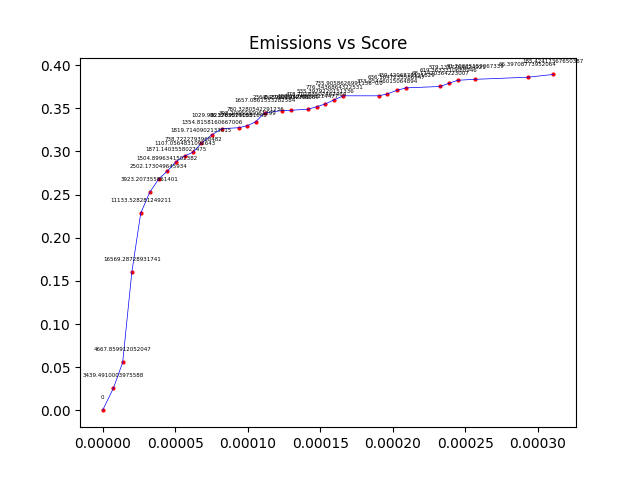
\includegraphics[width=0.6\textwidth, height=0.6\textheight]{images/curve_emissions_score.png}
        \caption{Andamento score e emissioni}
    \end{wrapfigure} 
Sull'asse delle x troviamo le emissioni, sull'asse delle y lo score. Quando la derivata è al di sotto di una certa soglia \textbf{S} per un certo numero di epoche consecutive \textbf{E} l'addestramento termina (comportamento asintotico).
Approssimazione della derivata della curva:
\begin{equation*}
    \frac{f(x_{i+1}) - f(x_i)}{x_{i+1} - x_i}
\end{equation*}
\end{frame}



\begin{frame}{RQ2 Addestramento sostenibile - Esplorazione}
    \begin{table}[H]
        \centering
        \resizebox{\textwidth}{!}{
        \begin{tabular}{|c|c|c|c|c|}
            \hline
            \textbf{Modello} & \textbf{Emissioni criterio classico (g)} & \textbf{Emissioni criterio nuovo (g)} & \textbf{Riduzione} & \textbf{\% riduzione emissioni} \\
            \hline
            DMF & 2.2927 & 1.97 & 0.32 & 14.21 \\
            \hline
            LINE & 1.91 & 1.38 & 0.53 & 27.69 \\
            \hline
            NGCF & 7.76 & 2.66 & 5.09 & 65.71 \\
            \hline
            DGCF & 94.90 & 10.46 & 84.44 & 88.97 \\
            \hline
        \end{tabular}
        }
        \caption{Esempi di confronto emissioni}
    \end{table}

    \begin{table}[H]
        \centering
        \resizebox{\textwidth}{!}{
            \begin{tabular}{|c|c|c|c|c|c|}
                \hline
                \textbf{Metrica} & \textbf{Modello} & \textbf{Score criterio classico} & \textbf{Score criterio nuovo} & \textbf{Riduzione} & \textbf{\% riduzione score} \\
                \hline
                \multirow{4}{*}{recall@10}
                                             & DMF & 0.14 & 0.14 & 0.0 & 0.0 \\ \cline{2-6}
                                             & LINE & 0.15 & 0.15 & 0.0 & 0.0 \\ \cline{2-6}
                                             & NGCF & 0.15 & 0.14 & 0.01 & 6.67 \\ \cline{2-6}
                                             & DGCF & 0.17 & 0.10 & 0.07 & 41.18 \\ \cline{2-6}
                \hline
            \end{tabular}
        }
        \caption{Esempi di confronto score}
        \label{tab:confronto-score}
    \end{table}
\end{frame}


\begin{comment}
\begin{frame}{RQ2 Addestramento sostenibile - Esplorazione}
 \begin{figure}[H]
    \centering
    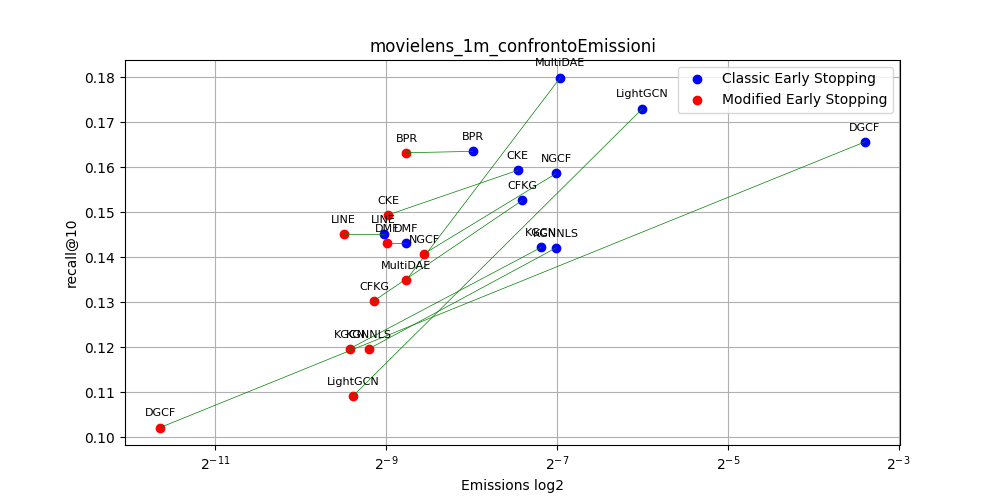
\includegraphics[scale=0.5]{images/recall@10_movielens_1m_comparison.png}
 \end{figure}
\end{frame}
\end{comment}



\begin{frame}{RQ3 Addestramento sostenibile - Confronto criteri}
    Sono stati eseguiti diversi esperimenti sul dataset MovieLens1M per confrontare diverse configurazioni dei parametri di soglia e di epoche, di seguito alcuni esempi\\
    \begin{table}[H]
        \centering
        \begin{tabular}{|c|c|c|c|}
            \hline
            \textbf{Modello} & \textbf{(Soglia,Epoche)} & \textbf{Riduzione emissioni} & \textbf{Riduzione score recall@10} \\ \hline
            \multirow{2}{*}{DMF} & (40,5) & 0.30 & 0 \\ \cline{2-4}
                                 & (30,7) &  0.31 & 0 \\ \hline
            \multirow{2}{*}{LINE} & (40,5) & 0.48 & 0 \\ \cline{2-4}
                                  & (30,7) & 0.47 & 0 \\ \hline
            \multirow{2}{*}{NGCF} & (40,5) & 5.0 & 0.02 \\ \cline{2-4}
                                  & (30,7) &  4.63 & 0.01 \\ \hline
            \multirow{2}{*}{DGCF} & (40,5) & 84.48 & 0.06 \\ \cline{2-4}
                                  & (30,7) & 81.52 &  0.05 \\ \hline
        \end{tabular}
        \caption{Esempi di risultati ottenuti}
    \end{table}
\end{frame}


\begin{frame}{RQ3 Addestramento sostenibile - Risultati confronto criteri}
\begin{table}[H]
    \scriptsize
    \centering
    \begin{tabular}{|c|c|c|}
        \hline
        \textbf{Modello} & \textbf{Parametro più impattante} & \textbf{Migliori risultati} \\
        \hline
        BPR & Soglia & Soglia 40 e 6 epoche \\
        \hline
        CFKG & Soglia & Soglia 40 e 6 epoche \\
        \hline
        CKE & Epoche consecutive & Soglia 40 e 6 epoche \\
        \hline
        DMF & Nessuno predominante & Soglia 40 e 7 epoche \\
        \hline
        KGCN & Epoche consecutive & Soglia 40 e 5 epoche \\
        \hline
        KGNNLS & Soglia & Soglia 40 e 5 epoche \\
        \hline
        LINE & Soglia & Soglia 40 e 7 epoche \\
        \hline
        MultiDAE & Soglia & Soglia 40 e 7 epoche \\
        \hline
        LightGCN & Soglia & Soglia 40 e 6 epoche \\
        \hline
        NGCF & Epoche consecutive & Soglia 40 e 5 epoche \\
        \hline
        DGCF & Epoche consecutive & Soglia 40 e 6 epoche \\
        \hline
    \end{tabular}
    \caption{Parametri più impattanti e migliori risultati per ciascun modello}
\end{table}
\end{frame}


\begin{frame}{RQ3 Addestramento sostenibile - Risultati confronto criteri}
\begin{table}[H]
    \scriptsize
    \centering
        \begin{tabular}{|c|c|c|c|}
            \hline
            \textbf{Tipo di Modello} & \textbf{Parametro predominante} & \textbf{Numero di Modelli} & \textbf{Modelli} \\ \hline
            Collaborative Filtering & Soglia & 5 & BPR, DMF, LightGCN, MultiDAE, LINE \\ \hline
            Collaborative Filtering & Epoche & 2 & NGCF, DGCF \\ \hline
            Knowledge Aware & Soglia & 2 & CFKG, KGNNLS \\ \hline
            Knowledge Aware & Epoche & 2 & CKE, KGCN \\ \hline
        \end{tabular}
    \caption{Riassunto dei parametri dominanti per tipo di modello}
\end{table}

\end{frame}